
\section{Ein einfaches Modell für einen \HR\ mit Substrat und 2DES}
\label{sec:cavity_model}

In Zusammenarbeit mit \name{V. Shikin} enstand ein einfaches und ein erweitertes theoretisches Modell für das System Elektronen im \HR. In diesem und im folgenden Abschnitt sollen diese nun vorgestellt und charakterisiert werden.

Mit Hilfe der Bewegungsgleichung von zweidimensionalen freien Elektronen \eqref{eqn:of_motion_real} und \eqref{eqn:of_motion_imag} ist es nicht möglich das vollständige Verhalten der Resonanz des \HR{}s vor allem für den Bereich hoher Elektronendichten zu erklären. Bisher fand hier nur ein störungstheoretischer Ansatz Verwendung, der für hohe Elektronendichten, wie sie auf dünnen Heliumfilmen vorliegen können, unter Umständen das Verhalten des Systems nicht mehr erklären kann. Um dieses Problem zu umgehen, wurde versucht eine analytische Lösung der Maxwell-Gleichungen für ein Modellsystem eines \HR{}s mit vereinfachter Geometrie zu finden.

Der hier vorgestellte Ansatz liefert eine Lösung der Maxwell-Gleichungen für das in Abbildung~\ref{fig:resshift_schema} skizzierte vereinfachte System. Da die Vereinfachungen des Modells mit der Realität nicht sehr viel gemeinsam haben, wird versucht nach jedem weiteren Schritt zu überprüfen, inwieweit das Modell noch physikalisch sinnvolle Ergebnisse liefert.

\begin{figure}[h!tbp]
	\centerline{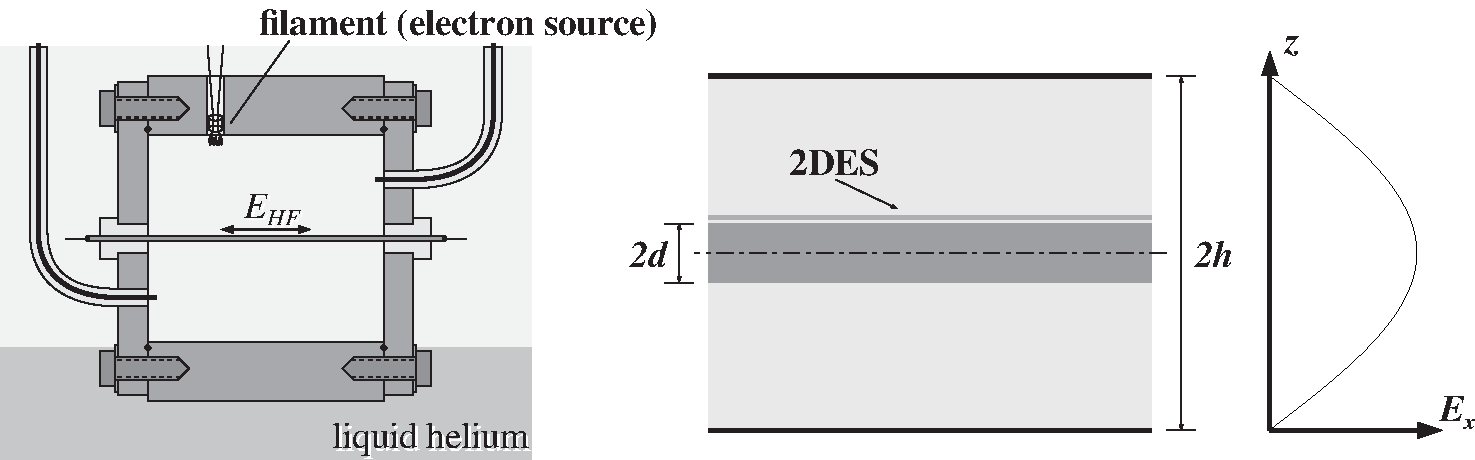
\includegraphics[width=0.8\textwidth]{theo_cavity/schema}}
	\caption[Vereinfachtes Resonatormodell]{Schema des im Text beschriebenen Modells der Messung von 2DES in einem Mikrowellen"=\HR. Es wird versucht den Resonator und die Ein- und Auskopplung der Messsignale zu modellieren. 
%	$\delta$ ist die 
%	%TODO was ist \delta
%	und $\varepsilon_1\ldots\varepsilon_3$ stellt eine Variation der Dielektrizitätskonstanten des Substrates dar.
}
	\label{fig:resshift_schema}
\end{figure}

Ausgegangen wird von einer in der $xy$-Ebene unendlich ausgedehnten Anordnung. Das elektrische Feld der TM$_\text{010}$-Mode wird durch folgende Funktion beschrieben, die die Randbedingung $\vec E=0$ an der \HR wand erfüllt. Für die Verteilung des elektrischen Feldes im Resonator gilt dann
	\begin{equation}
		\label{eqn:resshift_Edef}
		\vec E=E_0\begin{pmatrix}\sin\frac{\pi z}{h}\\
			0\\
			0\\\end{pmatrix}
		\ttextt{mit }
		\frac{\omega_0}{c}=\frac\pi{h}\quad.
	\end{equation}
In der Anwesenheit eines 2DES über dem Heliumfilm um das Substrat ergibt sich nach den Maxwell-Gleichungen dort ein Sprung im Magnetfeldanteil der \HR -Mode
	\begin{equation}
		H_y^\text{(Vakuum)}(d) - H_y^\text{(Substrat)}(d) = 4\pi j_x(d)/c\quad.
	\end{equation}
Hier sind $H_y^\text{(Vakuum)}(d)$ und $H_y^\text{(Substrat)}(d)$ die resultierenden Komponenten des Magnetfeldes im Vakuum und im Substrat. Für die Stromdichte $j_x(d)$ ergibt sich nach der Drude-Formel
	\begin{equation}
		j_x(d)=\sigma_{xx} E_x(d),\quad \sigma_{xx}=\frac{n_s e^2 \tau}
		{m_e^*(i\omega\tau + 1)}\quad.
	\end{equation}
Hierbei ist $\sigma_{xx}$ die diagonale Leitfähigkeit des 2DES und $m_e^*$ die
effektive Masse der Elektronen, die für Elektronen in einem 2DES auf flüssigem Helium näherungsweise mit ihrer Ruhemasse übereinstimmt.

Die Lösung des entsprechenden Eigenwertproblems führt zu folgender
Dispersionsgleichung:
	\begin{equation}
	\label{eqn:eigenfunction}
	k h\left[\tan(q d) - \frac{\sin{(k d)} + \cos{(k d)} \cot{(k h)}}{\cos{(k
	d)} - \sin{(k d)} \cot{(k h)}} \right]= i \frac{4 \pi}{c} \sigma_{xx}
	\end{equation}
Hierbei ist $\sigma = i\frac{4 \pi \sigma_{xx}}{c}$ die sogenannte
Kopplungskonstante, $k = \nicefrac{\omega}{c}$ die Wellenzahl im Vakuum und $q^2=\varepsilon_d\nicefrac{\omega^2}{c^2}$ die Wellenzahl im Substrat. Die Heliumfilmdicke auf dem Substrat ist für die Berechnung der Eigenmode zu vernachlässigen. Für die im Experiment
möglichen Werte von $n_s \approx \unit[10^8]{cm^{-2}}$ und $\tau \approx
\unit[10^{-7}]{s}$ ergibt sich ein Wert von $\sigma\approx1$. 

\begin{figure}[h!tbp]
	\includegraphics[width=\smidwidth]{theo_cavity/omega_sigma}%
	\hfill
	\begin{minipage}[b]{\textwidth-\smidwidth-\tabcolsep}
		\caption[Abhängigkeit der Resonanzfrequenz]{Die Abhängigkeit der \RF $\omega$ von der Kopplungskonstante $\sigma$ aus Gleichung~\eqref{eqn:eigenfunction}. Die \RF\ wird mit steigender Dielektrizitätskonstante reduziert.}
		\label{fig:cavity_eigenfunction}
	 \end{minipage}
\end{figure}

\subsection{Überprüfung des Modells}
%TODO
\label{ssec:check_model}

Zuerst einmal soll überprüft werden, inwieweit das oben vorgestellte Modell für einige einfache Grenzfälle sinnvolle Ergebnisse liefert.

\begin{description}
    \item[leerer Resonator mit flüssigem Helium:] Sinnvolle Werte für die Güte und die Frequenz der Resonanz. Einfüllen von flüssigem Helium verringert die \RF.
    \item[Resonator mit Substrat:] Die Anwesenheit eines dielektrischen Substrates reduziert die Resonanzfrequenz, weil dadurch die effektive Grösse der Resonators wächst und die Güte des Resonators erhöht sich, da die Energiedichte im Resonator steigt.
    \item[Resonator mit Substrat und 2DES:] ein 2DES wirkt wie eine dünne, schwach leitfähige Fläche im Resonator. Die Frequenz verschiebt sich nach oben und die Resonanz wird gedämpft.
\end{description}
Durch die aus Gründen der Vereinfachung nicht komplett an das Experiment angepassten Geometrie des Modells 

\section{Eine Erweiterung des Modells auf einen angekoppelten Resonator}
Um das Verhalten des hier verwendete \HR s genauer modellieren zu können, wurde das oben beschriebene Modell für einen einfachen Resonator auf einen Resonator mit Ankopplung an ein externes Mikrowellenfeld.
Diese Ankopplung des Resonators an externe ein- und auslaufende Mikrowellen wird durch eine variabel transparente obere Resonatorwand gewährleistet. 

Für die Reflexion $R$ der Anordnung erhält man folgende Gleichung:
\begin{equation}
\label{eqn:model_grund}
i(1 + R) + (1 - R) \left<\ldots\right> == i(\sigma_\text{re} - i \sigma_\text{im})(1 - R)
\end{equation}
hierbei ist der Teil $\left<\ldots\right>$ abhängig davon, welche in Abschnitt~\ref{ssec:check_model} angegebenen Variante des Modells Verwendung finden soll. 

\begin{description}
	\item[leerer Resonator mit flüssigem Helium:]
		Für diesen Fall gilt
		\begin{equation}
			\left<\ldots\right>=-\tan(h k)\quad.
		\end{equation}
		Die Reflexion $R$ des Resonators ergibt sich dann aus Gleichung~\eqref{eqn:model_grund}. 
	\item[Resonator mit Substrat:]
		Hier gibt es einen zusätlichen Anteil des Substrates mit der Dicke $d$ und der Auswirkung der Dielektrizitätskonstanten $\varepsilon$ auf $q=\sqrt{\varepsilon}k$. 
		\begin{equation}
			\left<\ldots\right>=\tan(d(k-q)-h k)
		\end{equation} 
	\item[Resonator mit Substrat und 2DES:]
		\begin{equation}
		-\left( \frac{i\,\Delta\sigma^\ast\,\cos(h\,k)+i\, \delta\sigma^\ast \,\sin(h\,k)+ 
		\sin (h\,k + d\,\left( -k + q \right) )}{i\,\delta\sigma^\ast\,\cos (h\,k) + \cos (h\,k + d\,\left( -k + q \right) ) - 
		i\,\Delta\sigma^\ast\,\sin (h\,k)} \right)
		\end{equation}
\end{description}

Die Lösung für die frequenzabhängige Transmission $T=1-R$des Resonators ergibt sich aus der Bestimmung von $R$ aus Gleichung \eqref{eqn:model_grund} in Abhängigkeit vom jeweils verwendeten Modell.

Unter \link{www.wuerl.net/CavityModel.html} kann ein Java Applet gestartet werden, in dem das Modell des Resonators mit Substrat und 2DES realisiert ist. 
